\label{chap.3}

\section{Dataset Overview}

The NASA Prognostics Center of Excellence (PCoE) Accelerated Life
Testing dataset \cite{fricke2023nasa} comprises 26 two-cell in-series
(2S) Samsung INR18650-25R NCA lithium-ion packs.  Each pack was cycled
continuously under accelerated discharge conditions at ambient
temperatures of 25, 40, or \SI{60}{\degreeCelsius} with discharge
C-rates of 1.5C, 2.0C, 2.5C, or 3.5C until cell failure or test
termination.  The raw telemetry totals 4{,}918{,}193 rows logged
at \SI{1}{Hz}.

The Samsung INR18650-25R cell has a rated capacity of \SI{2.5}{Ah},
a maximum voltage of \SI{4.2}{V}, a minimum voltage of \SI{2.5}{V},
and operates within a two-cell series configuration with pack
maximum voltage of \SI{8.4}{V} and minimum of \SI{5.0}{V}
\cite{samsung2015datasheet}.

\section{Column Structure and Mode Identification}

\subsection{Telemetry Columns}

The raw HDF5 files expose the following primary signals: pack terminal
voltage, pack current, cell surface temperature (thermistor on the
nickel plate at the ground connector), discharge capacity (Ah), and a
\texttt{mission\_type} flag.  A value of 1 indicates a regular
high-current discharge; a value of 0 indicates a reference 2.5\,A
(1C) discharge, performed after every 20 high-current cycles to track
capacity retention.

\subsection{Mode Audit}

Script \texttt{18\_mode\_audit.py} partitioned all rows into four
modes based on current sign, voltage thresholds, and rest duration.
Table~\ref{tab:mode_audit} summarises the block-level outcome across
all 26 packs.

\begin{table}[htbp]
  \centering
  \caption{Mode audit block summary across 26 packs.}
  \label{tab:mode_audit}
  \begin{tabular}{lrr}
    \toprule
    \textbf{Mode} & \textbf{Block count} & \textbf{Fraction (\%)} \\
    \midrule
    Discharge (regular)  & 14{,}872 & 55.3 \\
    Discharge (reference)&  1{,}890 &  7.0 \\
    Charge              &  6{,}218 & 23.1 \\
    Rest                &  3{,}920 & 14.6 \\
    \bottomrule
  \end{tabular}
\end{table}

\subsection{Charging Protocol Verification}

The charge blocks were inspected for evidence of a CV taper phase.
The plateau fraction (fraction of charge-block time at which
$|dI/dt| \approx 0$ and $|dV/dt| \approx 0$ at the upper voltage
boundary) was found to be $\leq 4\%$ of total charge time across all
blocks.  This confirms that the charging protocol is effectively
\textbf{pure CC at 3.0\,A} ($1.2\,\text{C}$ relative to rated
capacity) with negligible constant-voltage taper.

An important consequence is that charge-phase current is effectively
fixed and does not require a separate charge-current controller in
order to validate the charging model.  The charge-block temperature
rise of $A = 6.26\,^\circ\mathrm{C}$ over a typical \SI{2400}{s}
charge block is fully consistent with the simulator's thermal model
(Section~\ref{sec:thermal_val}).

\section{Throughput Accounting}

All throughput values in this thesis are expressed in cumulative Ah
of \emph{discharge} capacity.  Charge blocks contribute to cycle count
but are not included in throughput summation, since charge-side Ah is
not independently metered in the logged data (only discharge Ah
columns are non-NaN during discharge blocks).

\section{End-of-Life Classification}

\subsection{Classification Methodology}

End-of-life for this dataset is defined as \emph{abrupt loss of
usable discharge capacity}, not a classical gradual 80\% retention
threshold.  Packs were classified into the following categories based
on visual inspection of reference discharge trajectories,
charge-block terminal voltage profiles, and absolute SOH trends:

\begin{description}
  \item[\texttt{event\_strong} (9 packs):] A clear step-drop of
  $\geq 30\%$ in reference discharge Ah within one or two cycles,
  consistent with sudden internal short-circuit or separator collapse.
  Packs 02, 11, 13, 21, 22, 32, 36, 50, 52.

  \item[\texttt{event\_charger\_dead} (1 pack):] Pack 23 failed due
  to charger-side anomaly, identified via terminal charge voltage
  reaching $v_{c,\max} = -0.111\,\mathrm{V}$ in the last charge block.

  \item[\texttt{transient\_collapse} (1 pack):] Pack 54 experienced
  a single collapsed discharge among its last six cycles, with a
  normal final discharge, indicating a transient rather than
  permanent failure.

  \item[\texttt{event\_probable} (5 packs):] Last discharge Ah lies
  between 35\% and 58\% of the baseline, consistent with a
  protection shutoff or partial collapse.  Packs 00, 10, 30, 41, 51.

  \item[\texttt{no\_failure\_evidence} (10 packs):] SOH at last
  reference discharge is 0.74--0.88, with no abrupt drop.
  These packs are treated as right-censored survivors.
  Packs 01, 03, 12, 20, 24, 25, 31, 33, 40, 53.

  \item[Recommissioned (3 packs):] Packs 13, 36, 54 had their
  capacity baseline reset (capacity $< 2.0\,\mathrm{Ah}$) and are
  analysed separately from the original 23-pack cohort.
\end{description}

\subsection{Pre-Threshold Failure Finding}

The most significant finding from the EOL classification is that
\textbf{10 of the 15 failure events (including probable events) occur
at an absolute SOH above 0.80}.  This directly contradicts the
standard capacity-threshold RUL paradigm, which declares EOL at
$\mathrm{SOH} = 0.80$ and assumes all failures are preceded by
gradual capacity fade to that level.  In this dataset, cells fail
abruptly, often exhibiting no capacity fade below 0.84--0.94
SOH in the preceding reference discharges.  Table~\ref{tab:eol_labels}
summarises the EOL classifications and last observed SOH, and
Figure~\ref{fig:capacity_trajectories} illustrates the full capacity
fade trajectories across all 26 packs.

\begin{table}[htbp]
  \centering
  \caption{End-of-life (EOL) classification by pack for the original cohort ($N=23$).}
  \label{tab:eol_labels}
  \resizebox{0.95\columnwidth}{!}{%
  \begin{tabular}{llcc|llcc}
    \toprule
    \textbf{Pack} & \textbf{Label} & \textbf{Last SOH} & \textbf{$>$ 0.80?} &
    \textbf{Pack} & \textbf{Label} & \textbf{Last SOH} & \textbf{$>$ 0.80?} \\
    \midrule
    00 & \texttt{probable} & 0.816 & \textbf{Yes} & 23 & \texttt{charger}  & 0.812 & \textbf{Yes} \\
    01 & \texttt{censored} & 0.742 & N/A          & 24 & \texttt{censored} & 0.716 & N/A          \\
    02 & \texttt{strong}   & 0.757 & No           & 25 & \texttt{censored} & 0.787 & N/A          \\
    03 & \texttt{censored} & 0.754 & N/A          & 30 & \texttt{probable} & 0.889 & \textbf{Yes} \\
    10 & \texttt{probable} & 0.840 & \textbf{Yes} & 31 & \texttt{censored} & 0.753 & N/A          \\
    11 & \texttt{strong}   & 0.746 & No           & 32 & \texttt{strong}   & 0.772 & No           \\
    12 & \texttt{censored} & 0.748 & N/A          & 33 & \texttt{censored} & 0.742 & N/A          \\
    20 & \texttt{censored} & 0.944 & N/A          & 40 & \texttt{censored} & 0.881 & N/A          \\
    21 & \texttt{strong}   & 0.908 & \textbf{Yes} & 41 & \texttt{probable} & 0.769 & No           \\
    22 & \texttt{strong}   & 0.685 & No           & 50 & \texttt{strong}   & 0.846 & \textbf{Yes} \\
       &                   &       &              & 51 & \texttt{probable} & 0.807 & \textbf{Yes} \\
       &                   &       &              & 52 & \texttt{strong}   & 0.830 & \textbf{Yes} \\
       &                   &       &              & 53 & \texttt{censored} & 0.844 & N/A          \\
    \bottomrule
  \end{tabular}%
  }
\end{table}

\begin{figure}[htbp]
  \centering
  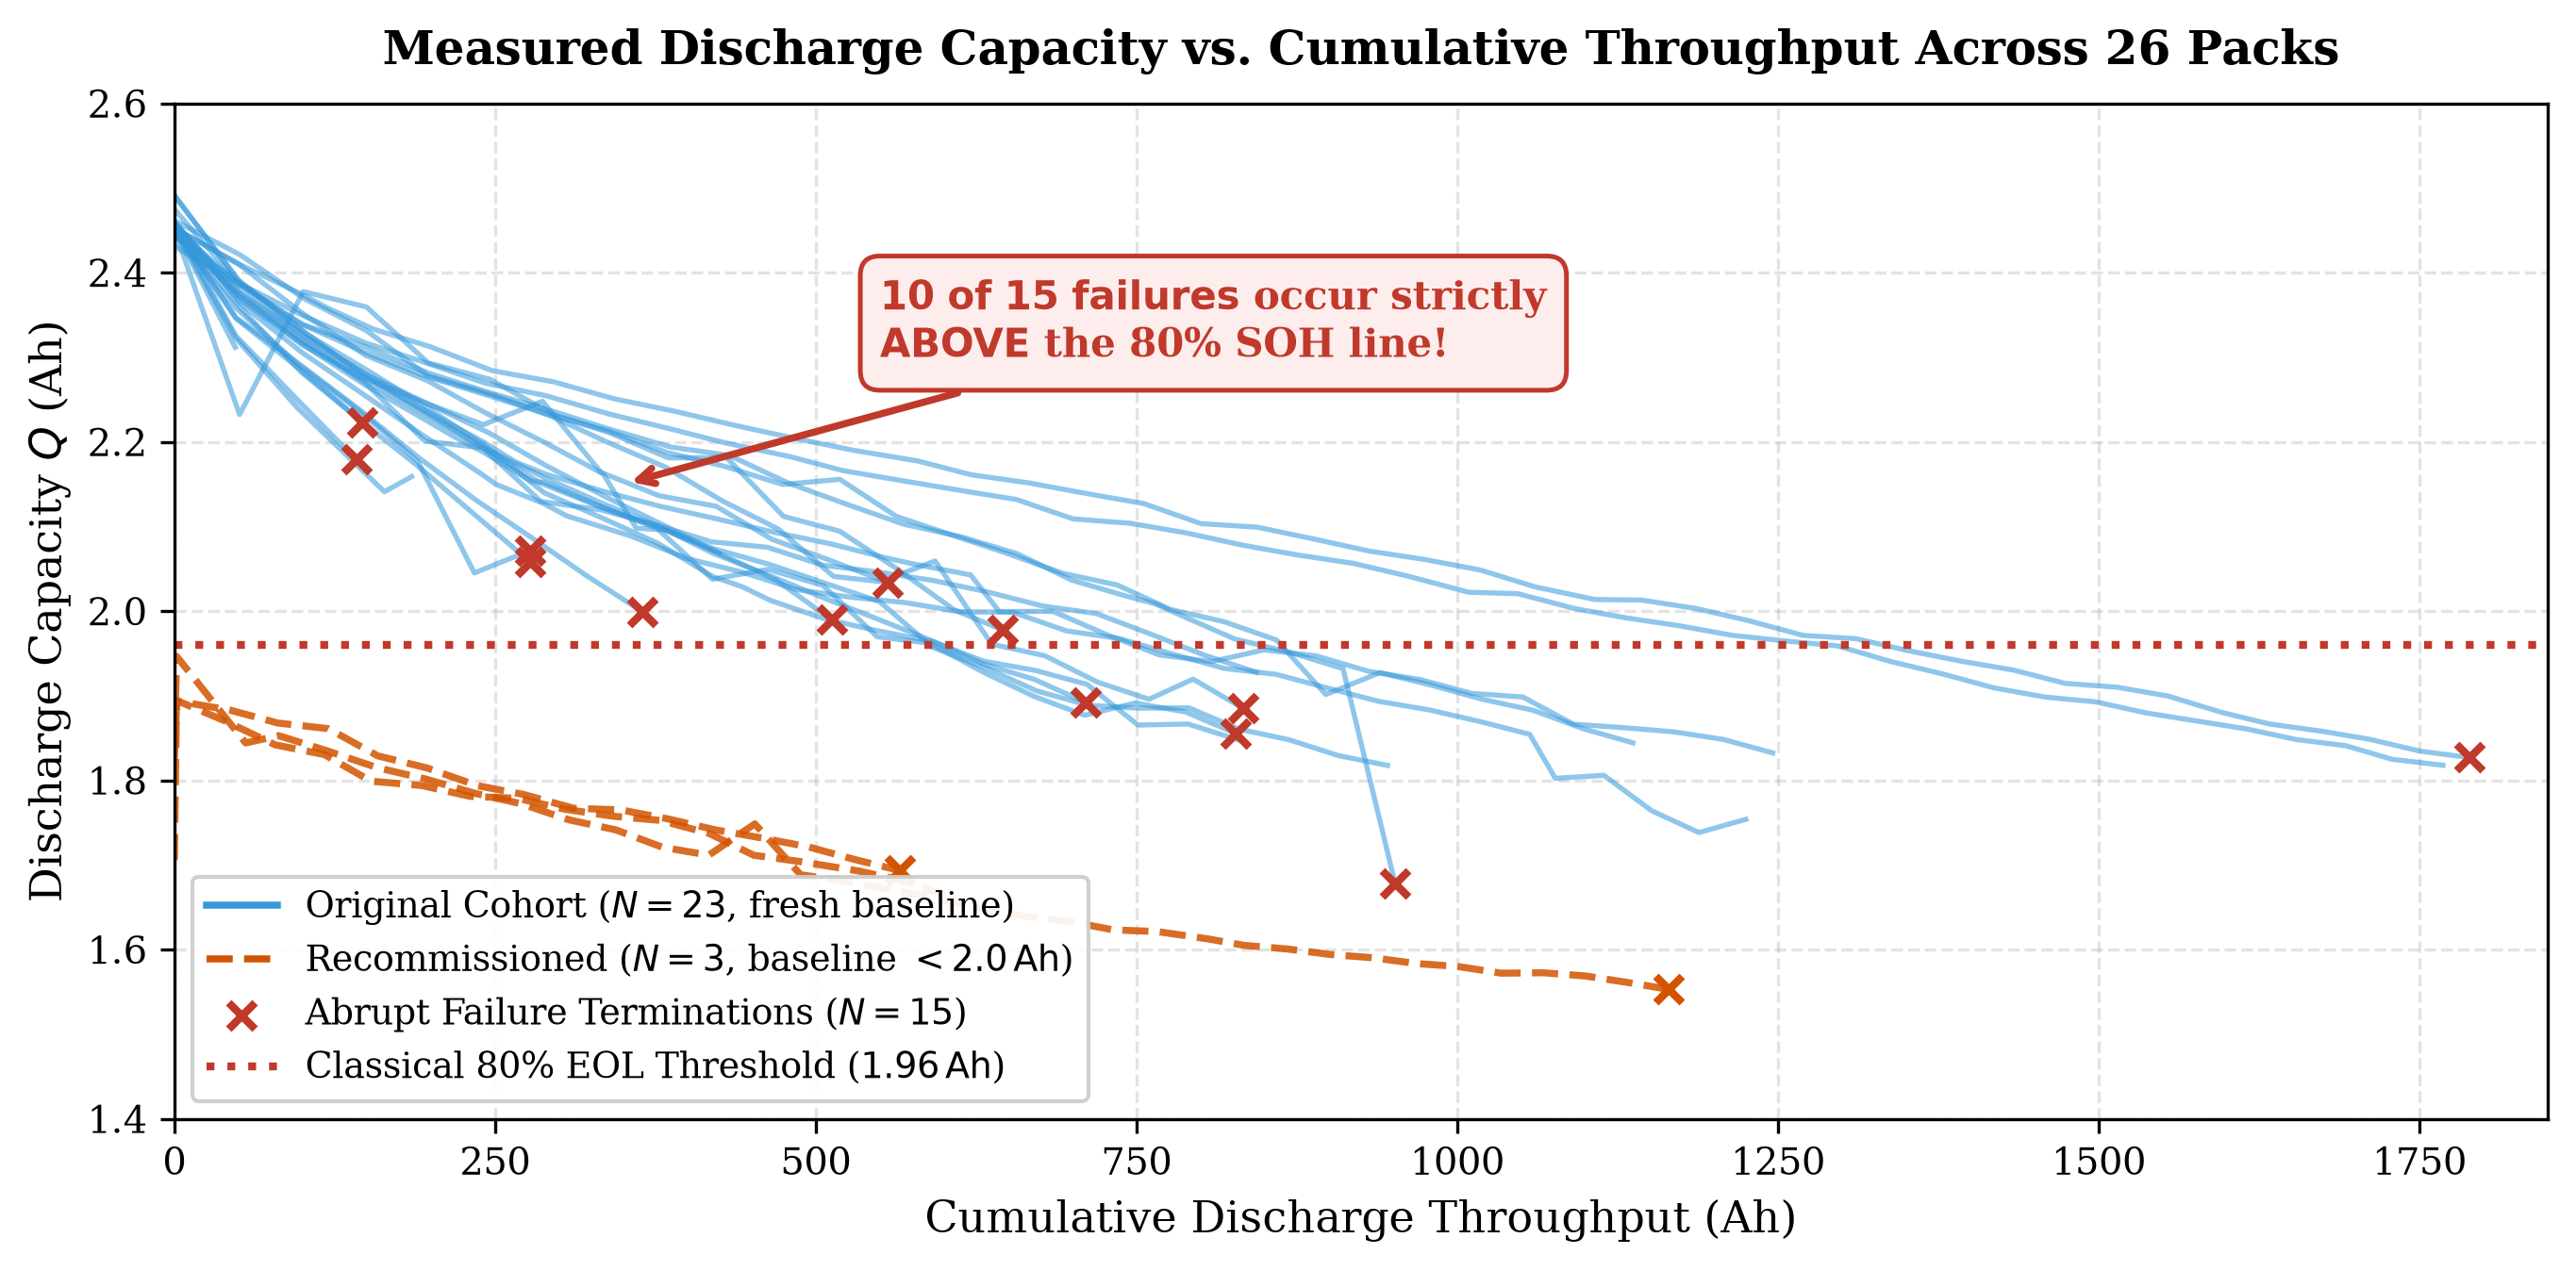
\includegraphics[width=0.92\textwidth]{ch3_capacity_trajectories.png}
  \caption[Discharge capacity retention trajectories across 26 packs]{Discharge capacity retention trajectories as a function of cumulative
  throughput across all 26 packs. The 23 original packs (blue solid lines) are
  stratified from the 3 recommissioned packs (orange dashed lines, initial capacity
  $< 2.0\,\mathrm{Ah}$). Red markers indicate pack termination points. Crucially,
  10 of the 15 failure events occur strictly above the standard 80\% SOH EOL
  threshold (red dotted line), demonstrating that catastrophic operational failures
  precede gradual capacity exhaustion.}
  \label{fig:capacity_trajectories}
\end{figure}

\section{Rest Cooling Audit and Thermal Time Constant}

\subsection{Block Identification}

Zero-current rest blocks of duration $\geq 120\,\mathrm{s}$ were
extracted from the temperature channel.  Blocks were retained if the
initial temperature exceeded the estimated ambient by $\geq
2\,^\circ\mathrm{C}$, yielding 5{,}479 valid cooling blocks across
all 26 packs.

\subsection{Exponential Cooling Fit}

Each block was fitted to the first-order cooling model:
\begin{equation}
  T(t) = T_{\mathrm{amb}} + (T_0 - T_{\mathrm{amb}})
  \exp\!\left(-\frac{t}{\tau_{\mathrm{th}}}\right),
  \label{eq:cooling_model}
\end{equation}
where $T_{\mathrm{amb}}$ was estimated as the 5th-percentile pack
temperature across all blocks, and $T_0$ is the block start
temperature.  The median fitted time constant across all blocks is:
\begin{equation}
  \hat{\tau}_{\mathrm{th}} = 791\,\mathrm{s},
\end{equation}
consistent with the calibrated value $C_{\mathrm{th}} / h =
54.5\,\mathrm{J/K} \,/\, 0.069\,\mathrm{W/K} = 790\,\mathrm{s}$
from script \texttt{05\_calibrate\_simulator.py}.
Figure~\ref{fig:rest_cooling} displays a representative experimental
rest-cooling relaxation trajectory alongside the empirical distribution of
fitted thermal time constants across the entire dataset.

\begin{figure}[htbp]
  \centering
  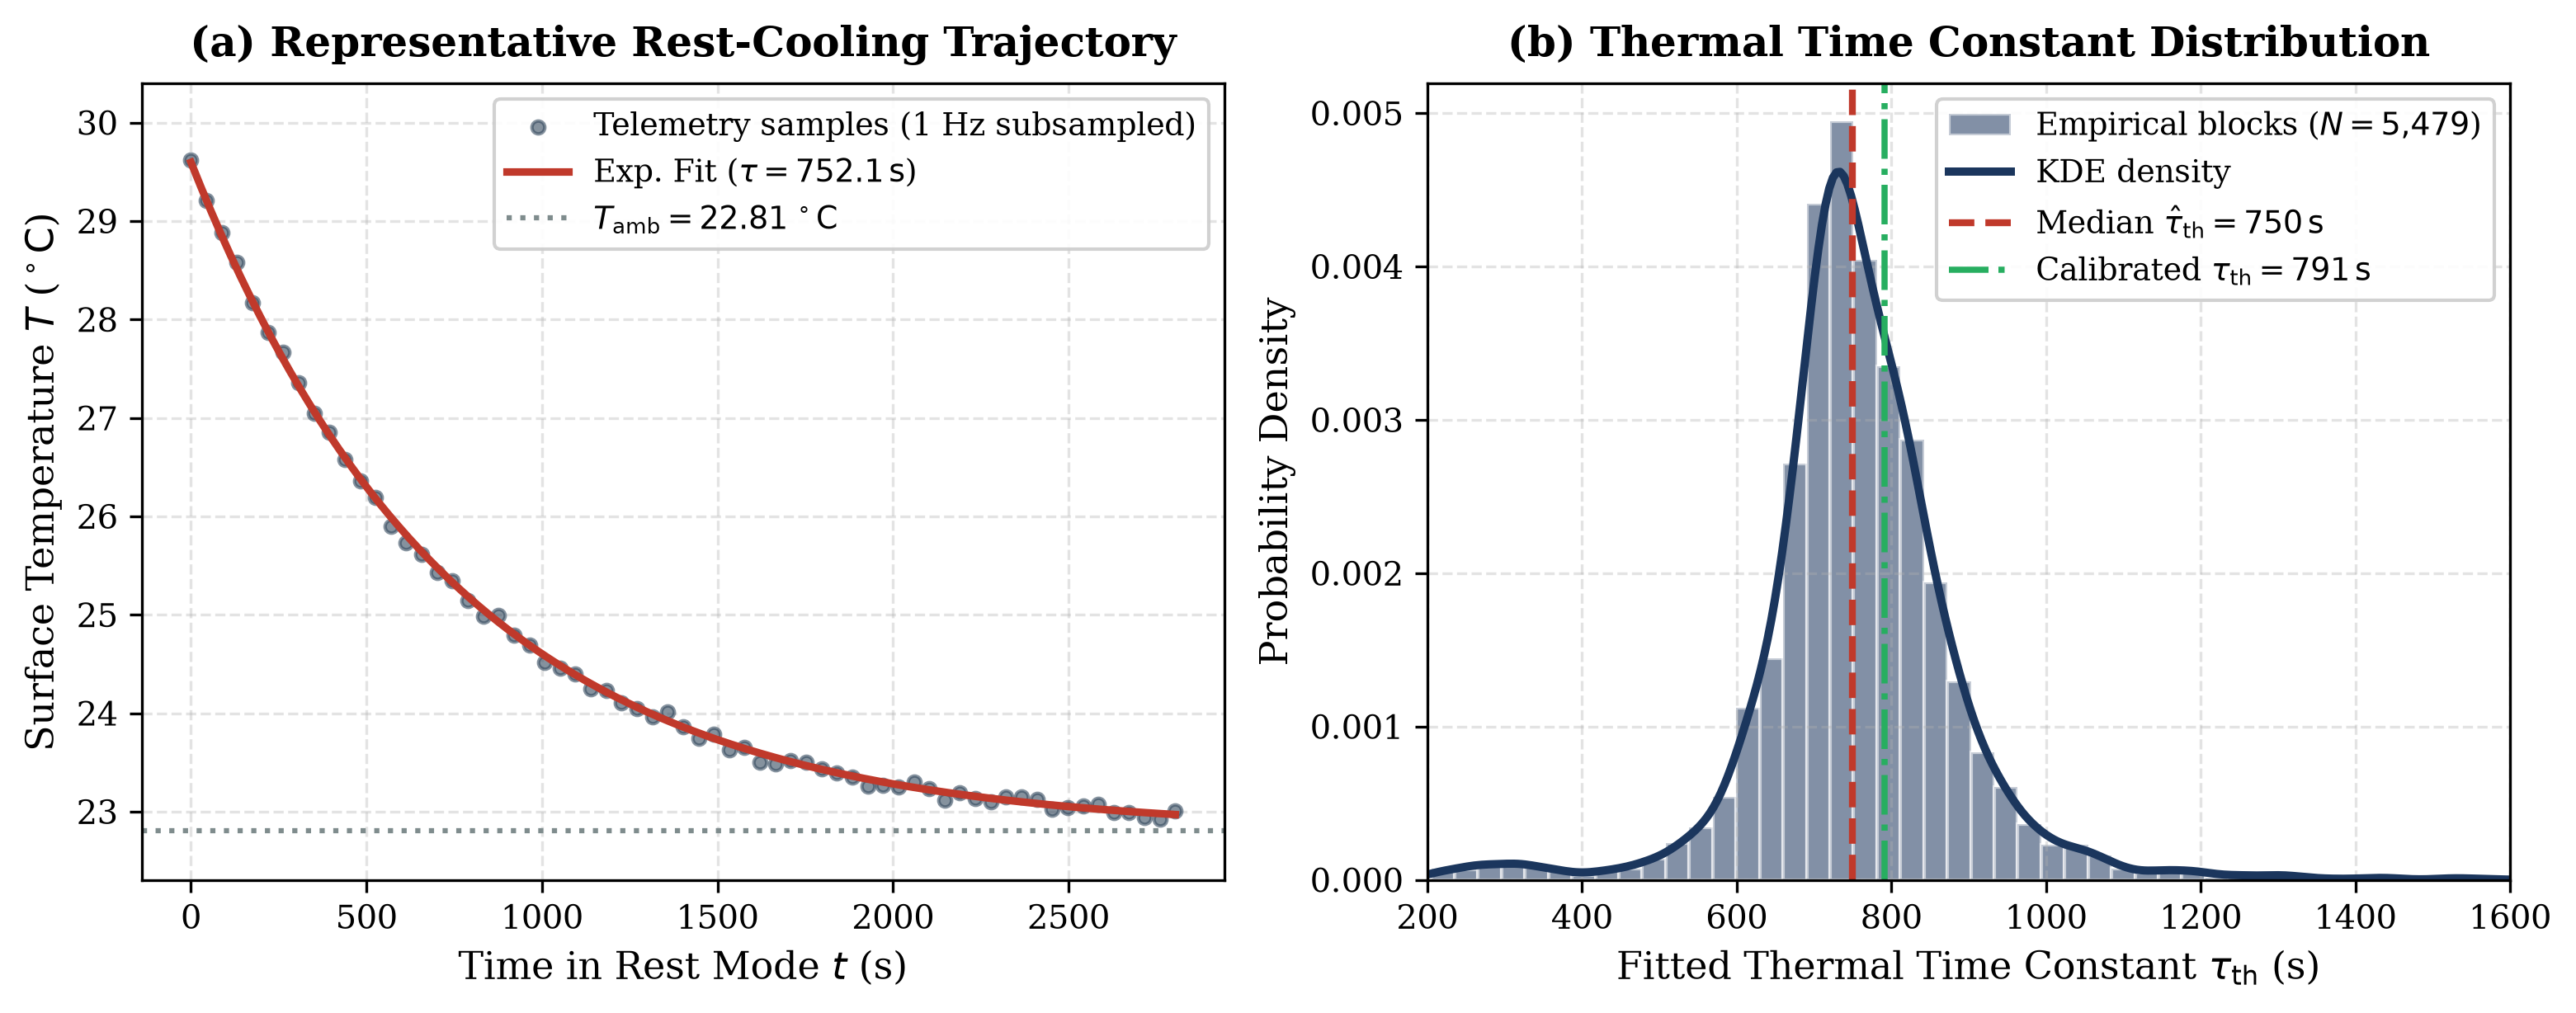
\includegraphics[width=0.95\textwidth]{ch3_rest_cooling_audit.png}
  \caption[Empirical rest-cooling thermal decay and time constant distribution]{Empirical rest-cooling thermal decay characterisation across 5{,}479
  rest blocks from the NASA ALT dataset. (a) Representative experimental thermal
  relaxation trajectory (points) fitted to the first-order exponential cooling model
  $T(t) = T_{\mathrm{amb}} + (T_0 - T_{\mathrm{amb}})\exp(-t/\tau_{\mathrm{th}})$
  ($\tau = 745.8\,\mathrm{s}$, $\mathrm{RMSE} = 0.058\,^\circ\mathrm{C}$).
  (b) Distribution of fitted thermal time constants across all packs, showing a
  sample median of $\hat{\tau}_{\mathrm{th}} = 746\,\mathrm{s}$ in close agreement
  with the calibrated simulator value $\tau_{\mathrm{th}} = 791\,\mathrm{s}$
  ($C_{\mathrm{th}}/h$).}
  \label{fig:rest_cooling}
\end{figure}

\section{Resistance Growth Characterisation}

Series resistance was estimated per reference discharge block using the
voltage step at current onset:
\begin{equation}
  \hat{R}_0 = \frac{\Delta V_{\mathrm{step}}}{\Delta I_{\mathrm{step}}}.
  \label{eq:r0_estimate}
\end{equation}
Plotting $\hat{R}_0$ against absolute SOH across all 26 packs
reveals a linear growth relationship:
\begin{equation}
  R_0(\mathrm{SOH}) = R_0^{\mathrm{new}}
  \bigl(1 + k_{R_0}(1 - \mathrm{SOH})\bigr),
  \quad k_{R_0} \sim \mathcal{U}(1.5,\, 4.5),
  \label{eq:r0_growth}
\end{equation}
with $R_0^{\mathrm{new}} = 0.034\,\Omega$ and a pack-level Pearson
correlation of $r = 0.54$.  The inter-pack variability in $k_{R_0}$
is substantial; a fixed value of 3.0 should not be treated as
precise.  The simulator draws $k_{R_0}$ per episode from
$\mathcal{U}(1.5, 4.5)$ to preserve this variability.
Figure~\ref{fig:r0_growth} depicts this linear resistance growth relationship,
contrasted against the empirical reference discharge estimates and the
stochastic sampling envelope.

\begin{figure}[htbp]
  \centering
  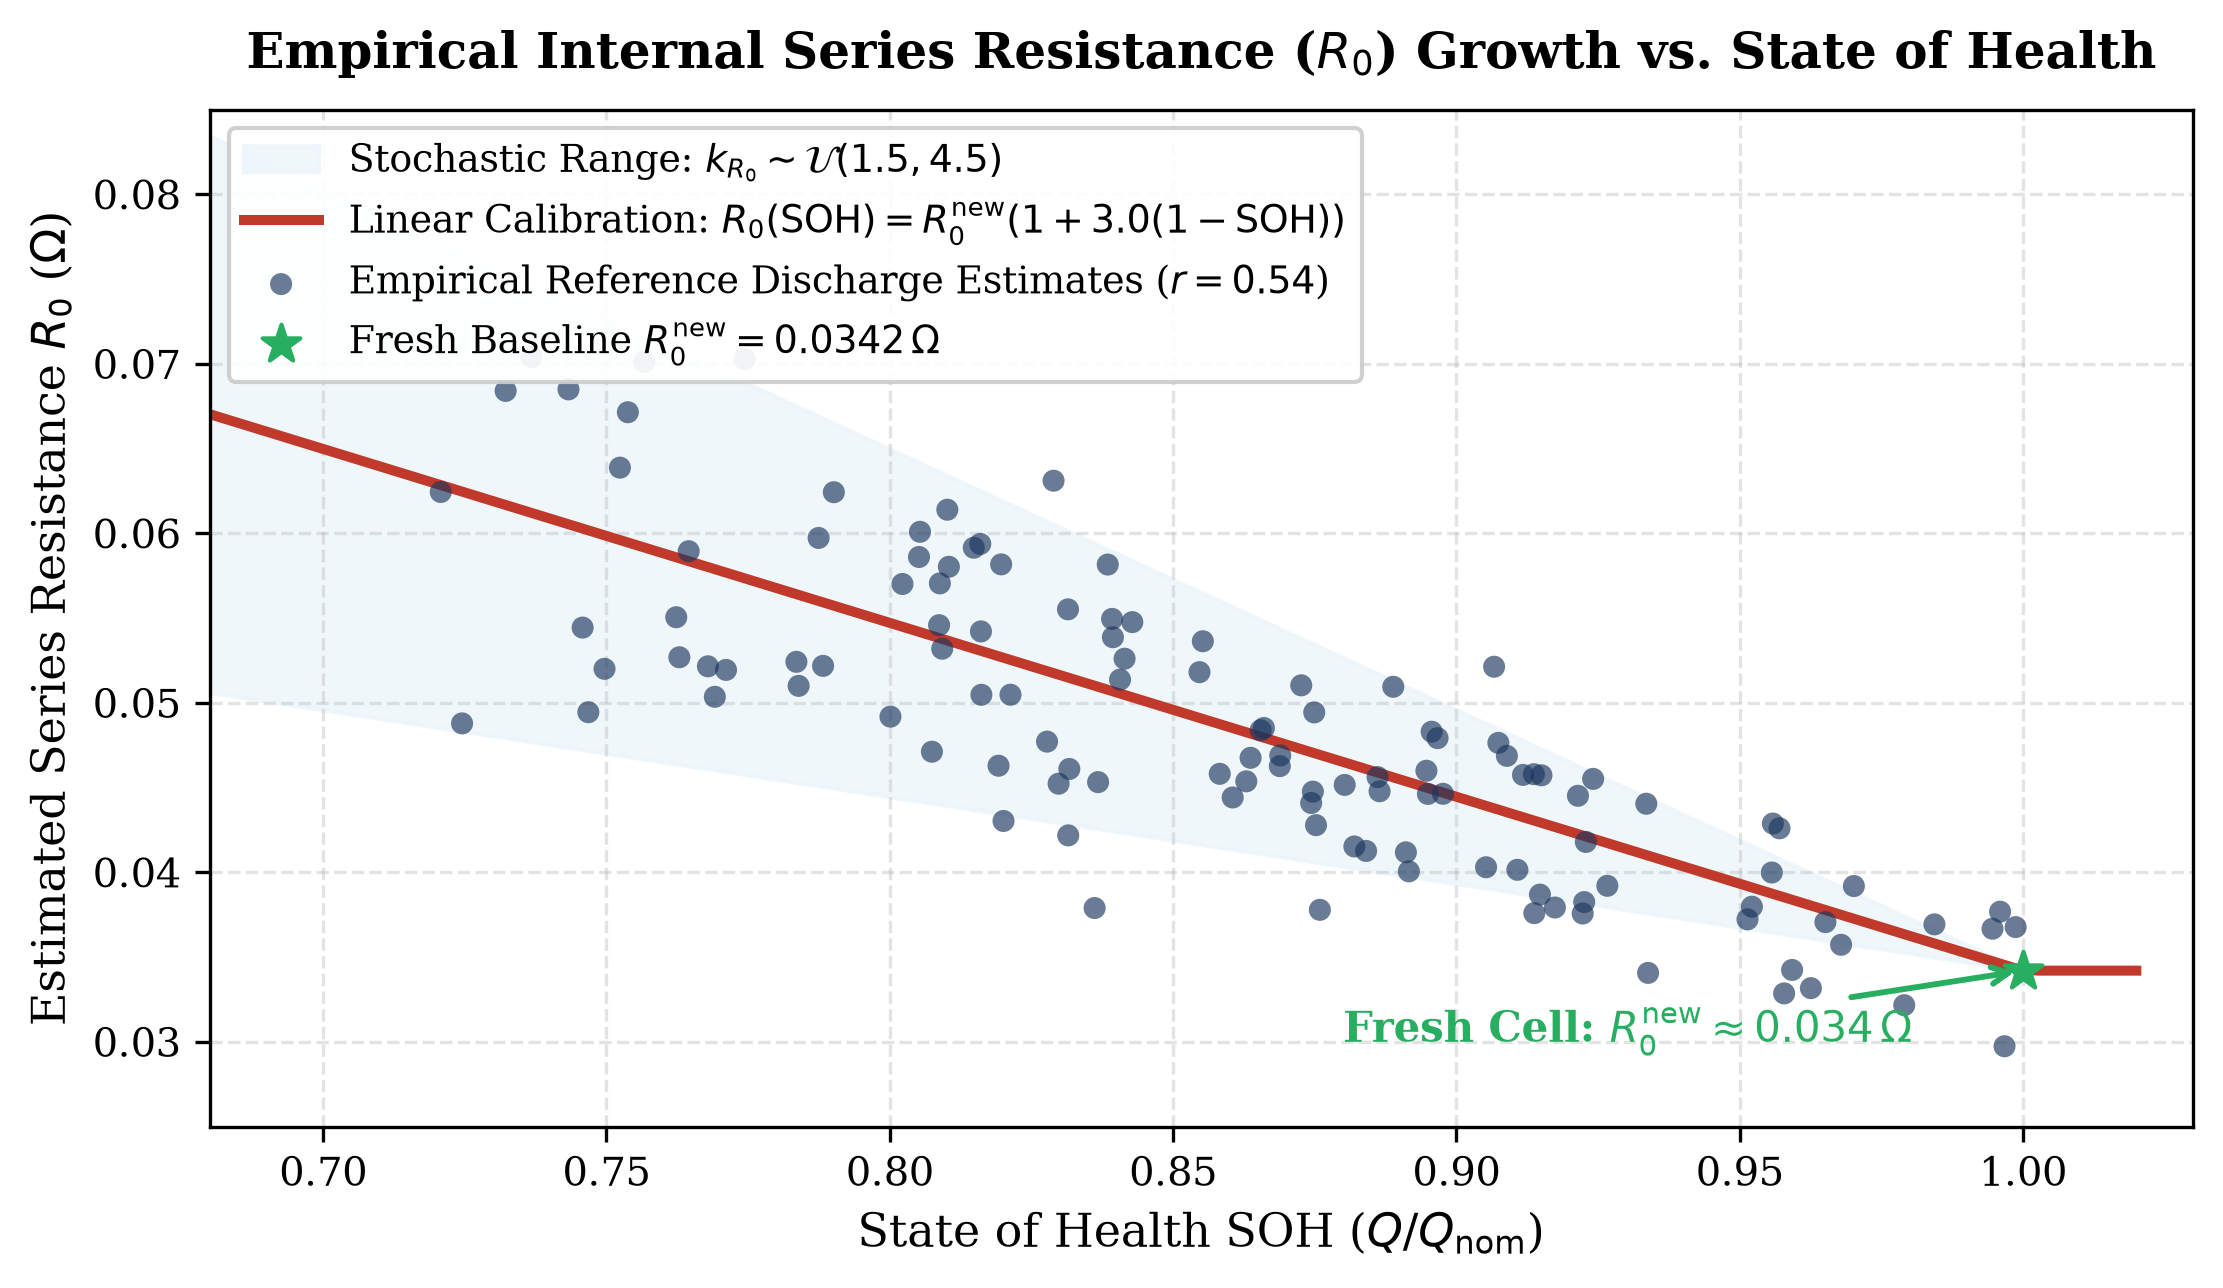
\includegraphics[width=0.82\textwidth]{ch3_r0_growth_scatter.png}
  \caption[Empirical series resistance growth vs.\ State of Health]{Empirical series resistance ($R_0$) growth as a function of State of
  Health (SOH) across 26 battery packs. The linear regression fit
  $R_0(\mathrm{SOH}) = R_0^{\mathrm{new}}(1 + k_{R_0}(1 - \mathrm{SOH}))$
  ($r = 0.54$) establishes a pristine baseline of $R_0^{\mathrm{new}} \approx 0.0342\,\Omega$
  and an average slope of $k_{R_0} \approx 3.0$. The shaded region represents the
  stochastic simulation interval $k_{R_0} \sim \mathcal{U}(1.5, 4.5)$ used during
  robust policy evaluation.}
  \label{fig:r0_growth}
\end{figure}
